\documentclass[12pt]{article}
%\usepackage[left=0.25cm,top=1cm,right=0.25cm,bottom=1cm]{geometry}
\usepackage{geometry}
\textwidth = 20cm
\hoffset = -1cm
\usepackage[utf8]{inputenc}
\usepackage[spanish,es-tabla]{babel}
\usepackage{amsmath}
\usepackage{nccmath}
\usepackage{amsthm}
\usepackage{amssymb}
\usepackage{graphicx}
\usepackage{color}
\usepackage{float}
\usepackage{multicol}
\usepackage{enumerate}
\usepackage{anyfontsize}
\usepackage{anysize}
\usepackage{enumitem}
\usepackage{capt-of}
\usepackage{bm}
\usepackage{relsize}
\usepackage{physics}
\usepackage{empheq}
\usepackage{mathtools}
\usepackage{bigints}
\usepackage{scalerel}
\spanishdecimal{.}
\setlist[enumerate]{itemsep=0mm}
\renewcommand{\baselinestretch}{1.2}
\let\oldbibliography\thebibliography
\renewcommand{\thebibliography}[1]{\oldbibliography{#1}
\setlength{\itemsep}{0pt}}
%\marginsize{1.5cm}{1.5cm}{0cm}{2cm}
%\renewcommand\theenumii{\arabic{theenumii.enumii}}
\renewcommand\labelenumii{\theenumi.{\arabic{enumii}}}

\def\scaleint#1{\vcenter{\hbox{\scaleto[3ex]{\displaystyle\int}{#1}}}}
\def\scaleoint#1{\vcenter{\hbox{\scaleto[3ex]{\displaystyle\oint}{#1}}}}
\def\scaleiiint#1{\vcenter{\hbox{\scaleto[3ex]{\displaystyle\iiint}{#1}}}}
\def\bs{\mkern-12mu}

\title{Ejercicios para el Tema 1 \\ \large{Matemáticas Avanzadas de la Física}}
%\subtitle{Fecha de entrega: 8 de marzo de 2016.}
\author{M. en C. Gustavo Contreras Mayén}
\date{ }

\begin{document}
\vspace{-4cm}

\maketitle
\fontsize{14}{14}\selectfont

\begin{enumerate}
\item Considera la transformación de coordenadas:
\begin{align*}
x = 2 \, u \, v, \hspace{1.5cm} y = u^{2} + v^{2}, \hspace{1.5cm} z = w
\end{align*}
Demuestra que el nuevo sistema de coordenadas \emph{es no ortogonal}.
\item Considera la transformación de coordenadas:
\begin{align*}
x = 2 \, u \, v, \hspace{1.5cm} y = u^{2} - v^{2}, \hspace{1.5cm} z = w
\end{align*}
Demuestra que el nuevo sistema de coordenadas \emph{es ortogonal}.
\item Escribe en coordenadas esféricas el siguiente vector:
\begin{align*}
\vb{A} = x \, y \, \vu{i} - x \, \vu{j} + 3 \, x \, \vu{k}
\end{align*}
adicionalmente expresa $A_{r}, A_{\theta}, A_{\phi}$ en términos de $r, \theta, \phi$.
\item Calcula las componentes rectangulares de la velocidad y aceleración de la partícula cuyo vector de posición está dado por:
\begin{enumerate}[label=\arabic{enumi}.\arabic*)]
\item $\vb{r} = A \, \cos n \, \omega \,  t \, \vu{i} + B \, \sin m \, \omega \, t \, \vu{j}$, con $n, m$ enteros.
\item $\vb{r} = 3 \, t \, \vu{i} - 4 \, t \, \vu{j} + \left( t^{2} + 3 \right) \, \vu{k}$
\end{enumerate}
\item Calcula las expresiones de las componentes polares de la velocidad y aceleración de las partículas cuyo vector bidimensional de posición está dado por:
\begin{enumerate}[label=\arabic{enumi}.\arabic*)]
\item $r = \dfrac{5}{2 - \cos \phi}, \hspace{0.5cm} \phi = \omega \, t$
\item $r = \dfrac{a}{t}, \hspace{0.5cm} \phi = b \, t$
\end{enumerate}
\item Para los siguientes ejercicios calcula $ds^{2}$, los factores de escala, el vector $\dd{\vb{s}}$, el elemento de superficie $\dd{\vb{S}}$, el elemento de volumen $\dd{V}$ y los vectores base $\vb{e}$, para cada uno de los siguientes sistemas coordenados:
\begin{enumerate}[label=\arabic{enumi}.\arabic*)]
\item  Coordenadas cilíndricas parabólicas:
\begin{align*}
x = \dfrac{1}{2} \left( u^{2} - v^{2} \right), \hspace{1.5cm} y = uv, \hspace{1.5cm} z = z
\end{align*}
cuyos dominios son:
\begin{align*}
u \in [-\infty, +\infty), \hspace{1cm} v \in (0, +\infty), \hspace{1cm} z \in (-\infty, +\infty)
\end{align*}
\item Coordenadas Esferoidales oblatas:
\begin{align*}
x &= a \, \sinh \xi \, \sin \eta \cos \phi \\[0.5em]
y &= a \, \sinh \xi \, \sin \eta \sin \phi \\[0.5em]
z &= a \, \sinh \xi \, \sin \eta
\end{align*}
cuyos dominios son:
\begin{align*}
\xi \in [0, +\infty), \hspace{1cm} \eta \in \left[ - \dfrac{\pi}{2}, \dfrac{\pi}{2} \right], \hspace{1cm} \phi \in [0, 2 \, \pi]
\end{align*}
\end{enumerate}
\item Demuestra que $\grad{\left( \phi \psi \right)} = \phi \, \grad{\psi} + \psi \, \grad{\phi}$
\item Si $f = f(r)$ con $r = \sqrt{x^{2} + y^{2}+ z^{2}}$, demuestra que:
\begin{align*}
\nabla{f(r)} = \vu{r} \, \dv{f(r)}{r}
\end{align*}
\item Demuestra que el campo eléctrico de una carga puntal:
\begin{align*}
\vb{E} = \dfrac{q \, \vu{r}}{4 \, \pi \epsilon_{0} \, r^{2}}
\end{align*}
cumple $\div{E} = 0$, para $r \neq 0$.
\item Evalúa las siguientes expresiones en coordenadas cilíndricas circulares:
\begin{align*}
\div{\vb{e}_{r}}, \hspace{1cm} \div{\vb{e}_{\theta}}, \hspace{1cm} \curl{\vb{e}_{r}},  \hspace{1cm} \curl{\vb{e}_{\theta}}
\end{align*}
\item Evalúa las siguientes expresiones en coordenadas esféricas:
\begin{align*}
\laplacian{r}, \hspace{1cm} \laplacian{\left( r^{2} \right)}, \hspace{1cm} \laplacian{\left( \dfrac{1}{r^{2}} \right)}, \hspace{1cm} \laplacian{\left( e^{i k r \cos \theta} \right)}
\end{align*}
\item El campo electrostático de un dipolo eléctrico $\vb{p} = p_{0} \, \vu{e}_{z}$ es:
\begin{align*}
\vb{E} = \dfrac{p_{0} (2 \, \vb{e}_{r} \, \cos \theta + \vu{e}_{\theta} \, \sin \theta)}{r^{3}}
\end{align*}
Demuestra que:
\begin{enumerate}[label=\arabic{enumi}.\arabic*)]
\item $\curl{\vb{E}} = 0$
\item para $r \neq 0$, se tiene $\div{\vb{E}} = 0$
\end{enumerate}
\item Usando coordenadas curvilíneas demuestra que:
\begin{align*}
\laplacian{(\phi \, \psi)} = \phi \, \laplacian{\psi} + \psi \, \laplacian{\phi} + 2 \, \grad{\phi} \vdot \grad{\psi}
\end{align*}
\item En una distribución tipo Maxwell la fracción de partículas moviéndose con velocidad $v$ y $v +\dd{v}$ es
\begin{align*}
\dfrac{\dd{N}}{N} = 4 \, \pi \left( \dfrac{m}{2 \, \pi \, k \, T} \right)^{3/2} \: \exp \left( - \dfrac{m \, v^{2}}{2 \, k \, T} \right) \: v^{2} \dd{v}
\end{align*}
donde $N$ es el número total de partículas. 
\par
El promedio o valor esperado de $v^{n}$ se define como:
\begin{align*}
\expval{v^{n}} = N^{-1} \scaleint{6ex} v^{n} \dd{N}
\end{align*}
Demuestra que:
\begin{align*}
\expval{v^{n}} = \left( \dfrac{2 \, k \, T}{m} \right)^{n/2} \dfrac{\left( \dfrac{n + 1}{2} \right) !} { \left( \dfrac{1}{2} \right) !}
\end{align*}
\item Se muestra en la figura (\ref{fig:figura_cicloide}) parte de una cicloide cuyas ecuaciones paramétricas son:
\begin{align*}
x &= a (\theta + \sin \theta) \\[0.5em]
y &= a (1 - \cos \theta)
\end{align*}
\begin{figure}[H]
    \centering
    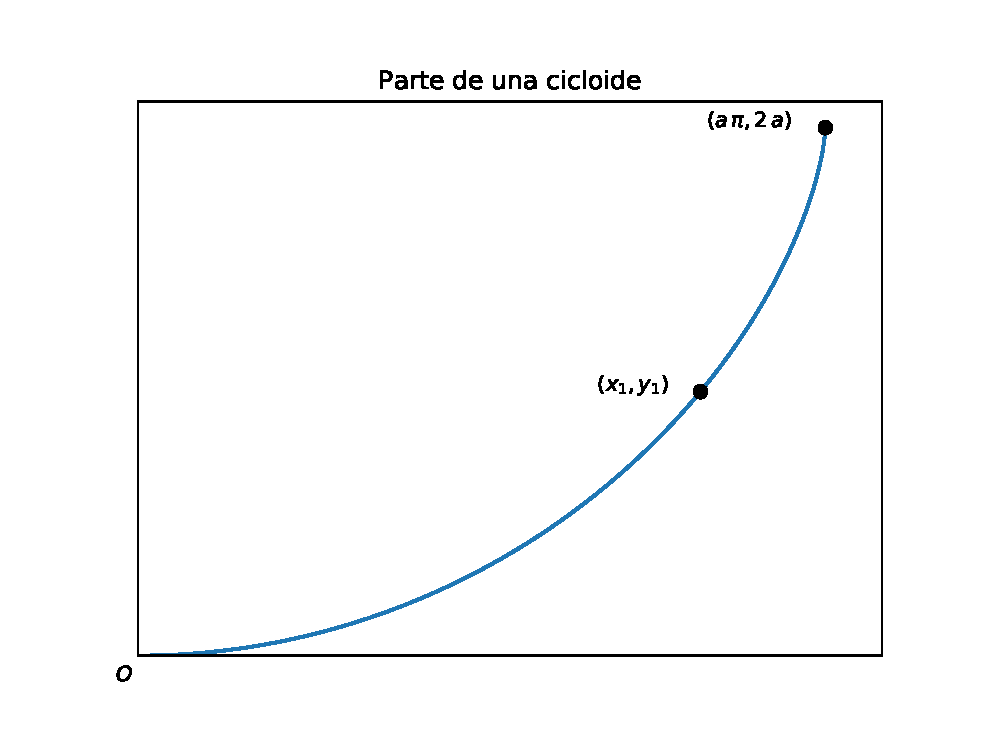
\includegraphics[width=0.75\textwidth]{Imagenes/plot_cicloide.eps}
    \caption{Una partícula deslizándose sobre una cicloide.}
    \label{fig:figura_cicloide}
\end{figure}
Demuestra que el tiempo que tarda una partícula para deslizarse sin fricción a lo largo de la curva desde el punto $(x_{1}, y_{1})$ hasta el origen, está dado por:
\begin{align*}
t = \sqrt{\dfrac{a}{g}} \, \scaleint{6ex}_{\bs 0}^{y_{1}} \dfrac{\dd{y}}{\sqrt{y \, (y_{1}- y)}}
\end{align*}
Sugerencia: Demuestra que la longitud del elemento de arco es:
\begin{align*}
\dd{s} = \sqrt{\dfrac{2 \, a}{y}} \dd{y}
\end{align*}
Evalúa la integral para demostrar que el tiempo es independiente de la posición inicial $y_{1}$.
\end{enumerate}
\end{document}